% L22rpo.tex
%
% Predrag created file				nov  2 2006
% $Author$ $Date$

\subsection{\Rpo s}

\ES{
The names of the \rpo\ figure files follow the convention
 {\tt rpoL-T-d.eps}s, with suffixes {\tt cm}
and {\tt u} indicating
 mean velocity frame  and $u$ representation respectively.
   }
%
Out of 30 \rpo s they
find,  only three are truly periodic.  The orbit
with $\period{p} = 95.25$ has a very small
$d = -6.5\,e^{-7}$, but it is not periodic 
(they
checked this by decreasing the integration step size and increasing the
number of modes).

The dynamics in this small system is competition between wavenumbers
2 and 3. The 2-\eqv\  and the 3-\eqv\  essentially lie in
the 2nd and 3rd Fourier component complex plane, with very
small deformations from higher harmonics.
Hence plot all \rpo s in these 2 representations:

$[ \Re a_2, \Im a_2, \Re a_3 ]$
(here 2-\eqv\  is a circle, 3-\eqv\ a vertical line)
 and
$[ \Re a_3, \Im a_3, \Re a_2 ]$
(here 3-\eqv\ is a circle, 2-\eqv\ a vertical line)

This stuff is hard to visualize... for ordinary periodic orbits one
plots the unstable plane of the \eqv, shows where the periodic
orbits sit. Other options:

Somewhat better visualization is in the
{\em mean velocity frame}, {\ie} 
a reference frame that rotates with with velocity 
$v_p=d_p/\period{p}$
In the mean velocity frame a \rpo\ becomes
a \po.
Mean velocity frame visualization helps quite a bit.
Put a black (green, respectively) dot
twice thicknes of the line every time unit; it will enable you to see
where the motion is slow and where it is fast.
% (a trick we used to understand plane Couette trajectories).
Mark the inital point on both
mean velocity \rpo\ and on \eqv\  in mean velocity
 frame with a fat triangle
indicating the direction, so we can see how they both move. Probably at the
opposite ends of the two curves - mean velocity frame is the mean motion.

%   rpo/figs/detail1rpo22-55-4.eps
%   rpo/figs/detail2rpo22-55-4.eps
%   rpo/figs/detail3rpo22-55-4.eps
%   break rpo22-55-4 into 3 parts.
%   The script for the fonts somehow crops these images

Each {\rpo} has its own mean velocity frame - and within it, {\eqv}
move on circles (or worse - because in higher Fourier modes they do mmore
complicted things), and it is important to know where the {\eqv} is at
a given instant.

As the shift $d$ is defined mod~$L$, better to
state for each {\rpo} its mean velocity $c_p = d_p/\period{p}$,
where $d_p$ is measured on the line (not on the circle). $c_p$ is
preferrable to angle $2\pi d_p/L$ as it does not vary in $L \to$~large 
limit (just like $\sqrt{2}$ wavelength estimate is independent of
system size.

The \rpo\ {\nameit}55 travels between the 2-\eqv\  and 
2-\eqv\ shifted,
with period and shift
$\period{p}=55.5953\,,\ d=5.24725$
Compared to $L/4 = 5.5$
this is nice, but why not close to periodic after 2nd return? Why 4th return?

The {\nameit}2 {\eqv}
captures qualitatively the mean velocity frame \rpo\ {\nameit}55 shape,
which follows the
{\eqv} for most of the time, except for a quick swing where it
sidesteps by $d/4$, just as it does in \reffig{f:rpo55}. 

\Rpo\ {\nameit}55 looks similar to Davidchack's  orbit
of period 
$\period{p}=47.64$ and $d=5.6759$. The period appears to depend on how
many times the orbit manages to spiral around the \eqv.
For {\nameit}55 that appears to be
1.5 times per period, rather than 2. This would led as
to
think there is a family of \rpo s along with a 3rd unit eigenvalue of
$gJ$,
but such does not exist.
So there has to be a selection mechanism corresponding to
reaching or missing the neighborhood of an \eqv\  point starting from
the neighborhood of the other. 

The $u$ space time evolution \reffig{f:rpo55u} % rpo22-55-4-u.eps 
is plotted with the same starting instant,
so one can also track also the spatial profile $u$ in parallel with
the Fourier space projections.

So it is almost impossible to see \reffig{f:rpo55}(b) %rpo22-55-4-cm.eps
in \reffig{f:rpo55}(a) % rpo22-55-4.eps.
I can see 4 periods in \reffig{f:rpo55}(a), %po22-55-4.eps,
but not in \reffig{f:rpo55}(b) %rpo22-55-4-cm.eps
where it comes back only after full period $\period{p}=55.6$.

It still seems that it could be made relative periodic 
(modulo a reflection symmetry?)
in $\period{p}/4=55.6/4=13.9$? That would be OK 
-
by symmetry the figure 8 connecting
2 symmetric {\eqva} could consist of 4 identical segments: from
{\eqv} A to midplane, then reflected version of the same to SA, and
back again.

\Eqv\ are solutions of 3-$d$ set of ODEs  \refeq{eq:3dks}, so
another convenient way to plot \eqva\ and \reqva\ on a periodic
domain $L$ is to plot 
$\partial u(x)$ vs. $u(x)$ as a curve parametrized by
$x\in [0,L]$. In this representation both \eqva\ and \reqva\ curves are
stationary, but the points on \reqva\ move as functions of time.

\Po s and \rpo s can be plotted this way as well
$\partial u(x,t)$ vs. $u(x,t)$. Now they are are represented by time-dependent
``tube".

\refFig{f:TW1TW2.ps}(b)
depicts the 2nd \REQV{+}{2}.
It belongs to the branch starting at point $M$
\PC{does it start at M?}
in bifurcation diagram \reffig{fig:GreeneKim}.
It has one real unstable eigenvalue = 0.337,
so it is more unstable than \REQV{+}{1},
but only in 1\dmn\ (\REQV{+}{1} is unstable in 4\dmn).
% Ruslan Feb 8 2007
\PC{please recheck this figure}


%%%%%%%%%%%%%%%%%%%%%%%%%%%%%%%%%%%%%%%%%%%%%%%%%%%%%%%%%%%%%%%%
\begin{figure}[t] %[h]
\centering
 	\includegraphics[width=0.50\textwidth]{figs/kse22_TW1_TW2.ps}
\hspace{0.1in}
\caption{
(a)
	\Reqv\ \REQV{+}{1}.
(b)
2nd \REQV{+}{2}, on the bifurcation branch starting
at point $M$ in \reffig{f:TW1TW2.ps},
and its decay into generic turbulence.
% Ruslan Feb 8 2007
        }
\label{f:TW1TW2.ps}
\end{figure}
%%%%%%%%%%%%%%%%%%%%%%%%%%%%%%%%%%%%%%%%%%%%%%%%%%%%%%%%%%%%%%%%%%


%%%%%%%%%%%%%%%%%%%%%%%%%%%%%%%%%%%%%%%%%%%%%%%%%%%%%%%%%%%%%%%%
\begin{figure}[t] %[h]
\centering
 	\includegraphics[width=0.18\textwidth]{figs/rpo22-55-4-u.eps}
\hspace{0.1in}
\caption{
 The \rpo\ {\nameit}55 in $u(x,t)$ representation. 
        }
\label{f:rpo55u}
\end{figure}
%%%%%%%%%%%%%%%%%%%%%%%%%%%%%%%%%%%%%%%%%%%%%%%%%%%%%%%%%%%%%%%%%%


%%%%%%%%%%%%%%%%%%%%%%%%%%%%%%%%%%%%%%%%%%%%%%%%%%%%%%%%%%%%%%%%
\begin{figure}[t] %[h]
\centering
(a) \includegraphics[width=0.44\textwidth]{figs/rpo22-55-4-clean.eps}
% ./removecache.sh rpo22-55-4.eps
% abandoned rpoEq22-55-4.eps with mean velocity equilibrium embeded.
%
\hspace{0.1in}
(b) \includegraphics[width=0.33\textwidth]{figs/rpoEq22-55-4-cm.eps}
\\
(c) [create rpoEq22-55-4-cm-?.eps]
\caption{
 The \rpo\ {\nameit}55 in: 
 (a) Phase space, traced for four periods $\period{p}$.
% Green curve belongs to \reffig{f:rpo55}(b) % rpo22-55-4-cm.eps
% rather than to  \reffig{f:rpo55}(a), % rpoEq22-55-4.eps?
 (b) mean velocity frame. 
        The continuos family of 
	{\eqva} A obtained by the action of $g$ is shown in green,
	the SA family shown in red. The \rpo\ {\nameit}55 stays close
	to either A or SA for close to 1/2 of {\eqv} rotation
	period, then quickly jumps to the other {\eqv} point.
 (c) mean velocity frame A, SA and {\nameit}55 projected on the 
	$[a_?,a_?]$ plane,
	with the $\sigma x = -x$ symmetry of \KSe\ explicit.
        }
\label{f:rpo55}
\end{figure}
%%%%%%%%%%%%%%%%%%%%%%%%%%%%%%%%%%%%%%%%%%%%%%%%%%%%%%%%%%%%%%%%%%


The two {\eqva}
capture qualitatively the mean velocity frame \rpo\ {\nameit}55 shape,
which follows the
{\eqv} for most of the time, except for a quick swing where it
sidesteps by $d/4$, just as it does in \reffig{f:rpo55}. 

Please also plot it in plane, chose small Fourier coefficients
 which respect the $x \to -x$ symmetry of \KSe.
Then the symmetry of 2 mean velocity
{\eqva} and self-dual symmetry of \rpo\ {\nameit}55 will be explicit.

Eigenvalues of \rpo\ {\nameit}55 $g\jMps$: are
\\
$(-57.17,  1, 1, -0.500, -0.012, \cdots)$ .
%
%  Eigenvalues of the Jacobian without rotation
%  84.15, -33.86 + 28.94 i, c.c. , 0.48, 0.00019
% no good - missing marginal ones

plots:
  76 rpo60fm23.jpg	\\
 909 rpo60fm23.emf	\\
% Ruslan L Davidchack, 	10 Jul 2006 
the 55 rpo, or whichever seems easiest to explain:
$\period{} = 59.89$,
$c_p = d_p/\period{p}= ?$

$(\ExpaEig_i e^{\pm i\theta_i})=
(
\\
 -27.03397007874626,
\\
   9.34426620337976,
\\
   1
\\
   1
\\
  -0.05018967056231,
\\
   0.00015065158255,
)$

The eigenvectors
indicate that an amplitude mode comes paired with the 
group shift-invariant mode $\ExpaEig_4 =1$. It probably says that
the amplitude $|u_k|$ of the associated can be easily perturbed (think of
a large system: $|u(x)|$ can be easily deformed by long wavelength
perturbations. This \underline{must} be understood. Proposal:

There are two
marginal eigenvalues, one for time translation, one for
rotational invariance. 
The sign of $\ExpaEig_{1}=-57$ says this is a Moebius-kind orbit,
inverse hyperbolic.
Stability exponent
 $\eigExp[1]=0.07$ says that this neighborhood is much less repelling than
the central {\eqv} A, a better candidate for being embedded into the
ergodic attractor.

The \rpo\ initial condition is
so accurate the orbit in \reffig{f:rpo55}(b)
start visibly deviating after retracing the loop 6.5 times.
% the largest unstable multiplier is 
% $-57.17$ per period of the orbit - error would grow to $\approx 60^7
% = 2,800,000,000,000$.

For the \rpo s the accuracy of Jacobian depends
on the time step size, and long runs are needed to refine the results

For a numerical check of the \rpo\ stability eigenvalues,
used two inital
points along an unstable eigenvector $\jEigvec{1}$
at radial distance  $\approx 10^{-4}$ from the \eqv\ {\nameit}2,
and the initial inter-point separation $\Delta(0) \approx 10^{-5}$.
Integrated for time equal to the period $\period{p}=26.3556$ as calculated from
the \jacobianM\ and computed the leading Lyapunov exponent from the ratio of
final to initial distance 
$\Lyap= {1 \over \period{}}\ln( \Delta(\period{})/\Delta(0))$.
Get
$\Delta(\period{})/\Delta(0) =39.01$,
$\Lyap=0.13902$, in agreement with the \eqv\ {\nameit}2 
expanding eigenvalue $\Lyap=0.13904$
\[
\ExpaEig_{radial} =  e^{\Lyap \period{}} =38.99
\,.
\]

% Ruslan L Davidchack, 	10 Jul 2006 
The orbit RLD found has period 60 
rather than 55.  Because it comes so close to the steady states, 
this is probably a numerical precision error.
\\
plots:
 180 rpos1.jpg	\\
1594 rpos1.emf	\\


Rewrite Fourier modes as $u_k(t) = e^{r_k(t) + k(\theta_k(t))}$, study
dynamics and Jacobinas in the $\dot{r_k},\dot{\theta_k})$ representation.
\nameit 2 and \nameit 3 \eqva\ are nearly cirlces in this representation - higher
modes will not wind wildly if represented by $\theta_k(t)$? Kind of WKB
representation.

period 77 rpo jumps between the two steady states.
\\
plots:	\\
  84 rpo77fm23.jpg	\\
1133 rpo77fm23.emf	\\
 176 rpos2.jpg	\\
1594 rpos2.emf	\\

